\documentclass[10pt]{beamer}
\usepackage{makecell}
\usepackage{amssymb,amsmath}
\usepackage{graphicx}
\usepackage{url}
\usepackage{color}
\usepackage{pagenote}[continuous,page]
\usepackage{relsize}		% For \smaller
\usepackage{url}			% For \url
\usepackage{epstopdf}	% Included EPS files automatically converted to PDF to include with pdflatex

%For MindMaps
% \usepackage{tikz}%
% \usetikzlibrary{mindmap,trees,arrows}%

%%% Color Definitions %%%%%%%%%%%%%%%%%%%%%%%%%%%%%%%%%%%%%%%%%%%%%%%%%%%%%%%%%
%\definecolor{bordercol}{RGB}{40,40,40}
%\definecolor{headercol1}{RGB}{186,215,230}
%\definecolor{headercol2}{RGB}{80,80,80}
%\definecolor{headerfontcol}{RGB}{0,0,0}
%\definecolor{boxcolor}{RGB}{186,215,230}

%%% Save space in lists. Use this after the opening of the list %%%%%%%%%%%%%%%%
%\newcommand{\compresslist}{
%	\setlength{\itemsep}{1pt}
%	\setlength{\parskip}{0pt}
%	\setlength{\parsep}{0pt}
%}

%\setbeameroption{show notes on top}

% You should run 'pdflatex' TWICE, because of TOC issues.

% Rename this file.  A common temptation for first-time slide makers
% is to name it something like ``my_talk.tex'' or
% ``john_doe_talk.tex'' or even ``discrete_math_seminar_talk.tex''.
% You really won't like any of these titles the second time you give a
% talk.  Try naming your tex file something more descriptive, like
% ``riemann_hypothesis_short_proof_talk.tex''.  Even better (in case
% you recycle 99% of a talk, but still want to change a little, and
% retain copies of each), how about
% ``riemann_hypothesis_short_proof_MIT-Colloquium.2000-01-01.tex''?

\mode<presentation>
{
  \usetheme{CambridgeUS}
  \usecolortheme{dolphin}
  \useoutertheme{default}
  \useinnertheme{default}
  \setbeamercovered{invisible} % or whatever (possibly just delete it)
}
\beamertemplatenavigationsymbolsempty

\usepackage[english]{babel}
%\usepackage[latin1]{inputenc}
\usepackage{subfigure}

\usepackage{times}
\usepackage[T1]{fontenc}
\usepackage{CJKutf8}

%% makes the ppagenote command for figure references at the end.
\makepagenote
\renewcommand{\notenumintext}[1]{}
\newcommand{\ppagenote}[1]{\pagenote[Page \insertframenumber]{#1}}

\title[Experiment Design (01CH740)]{Experiment Design for Computer Sciences (01CH740)}
\author[Claus Aranha]{Claus Aranha\\{\footnotesize caranha@cs.tsukuba.ac.jp}}
\institute[U. Tsukuba]{University of Tsukuba, Department of Computer Sciences}



% TODO: this class needs more real examples from real data.


\title[]{Experiment Planning and Design}
\subtitle[]{Lecture 6: Techniques for Hypothesis Testing, Part II}
\author[Claus Aranha]{Claus Aranha\\{\footnotesize caranha@cs.tsukuba.ac.jp}}
\institute{Department of Computer Science}
\date{2015-06-09}

\begin{document}

\section{Introduction}
\subsection{Outline}

\begin{frame}
  \maketitle
\end{frame}


\begin{frame}
  \frametitle{The story so far...}
  % TODO: review of the classes so far
\end{frame}

\begin{frame}
  \frametitle{Outline for this class}
  \begin{block}{}
    A few more techniques for dealing with special experiments
  \end{block}
  \begin{itemize}
  \item Paired Testing;
  \item ANOVA;
  \item Model Selection (Parameter Selection);
  \end{itemize}
\end{frame}

\section{Paired Testing}

\subsection{Paired Tests}

\begin{frame}
  \frametitle{Paired Design}
  \begin{block}{Imagine this situation}
    A scientist develop an optimization algorithm, $A$, for a family
    of problems, and wants to compare its convergence speed against
    the state-of-art algorithm, $B$.

    \medskip

    The Researcher implements both methods, and wants to determine
    whether the proposed one has a better average performance for
    problems of that particular family.

    \medskip

    The measurements are made under homogeneous conditions (same
    computer, same operational conditions, etc). And the running time
    is measured in a way that is not sensitive to other processes
    running in the system.
  \end{block}
\end{frame}

\begin{frame}
  \frametitle{Dependent Populations}
  This problem has some important questions worth considering:
  \bigskip

  \begin{itemize}
  \item What is the actual question of interest?
  \item What is the population for which this question is interesting?
  \item What are the independent observations for that population?
  \item What is the relevant sample size for the experiment?
  \end{itemize}
  
  \bigskip

  Please think a little and propose answers to these questions.
\end{frame}

\begin{frame}
  \frametitle{Paired Design} 

  The variability due to the different test problems is a strong
  source of spurious variation that \structure{can and must} be
  controlled.

  \medskip

  An elegant solution to eliminate the influence of this nuisiance
  parameter is the pairing of the measurements by problem:
  
  \medskip

  \begin{itemize}
  \item Observations are considered in pairs (A,B) for each problem.
  \item Hypothesis testing is done on the sample of \emph{differences}
  \end{itemize}
  
\end{frame}


\begin{frame}
  \frametitle{Another example (1)}
  \begin{columns}[c]
    \column{0.3\textwidth}
    
\includegraphics[width=1\textwidth]{img/soccer}
    \column{0.7\textwidth}
    \begin{block}{}
    How would you test the differences between two types of shoes (A and B)?
    \end{block}
    \begin{enumerate}
    \item<2> Give some kids the shoe A, and some kids the shoe B\\ 
      {\small The personality of the kid becomes a factor -- more agressive
      kids may wear the shoe faster?}
    \item<2> Give each kid one of each shoe: Left shoe A, right shoe B (or random)\\
      {\small In this way each kid will use both shoes equally.}
    \end{enumerate}
    \begin{block}{}
      Can we use this information (same kid used both shoes) to
      improve our statistical testing?
    \end{block}
    \vfill

    \hfill{\tiny Image from http://leagueathletics.com/}
  \end{columns}
\end{frame}

\begin{frame}
  \frametitle{Paired Tests (2)}
  \begin{block}{Interface Testing}
    Imagine you are comparing two HCI technologies using a survey. You
    ask each surveyed person to compare two systems using a score.
  \end{block}
  \bigskip

  \begin{itemize}
  \item Scores given by the same person should show the same biases;
  \item Thus, you want to compare the scores described by the same voters;
  \item \alert{Important!} Don't forget to change the order of voting!
  \end{itemize}
\end{frame}

\begin{frame}[fragile,singleframe]
  \frametitle{Paired T-Test}
  \begin{itemize}
  \item The Paired T-test is based on the idea of calculating the
    difference between the samples. 
  \item This difference is then treated as
    a one-sample test.
  \end{itemize}
  \begin{block}{}
{\small
\begin{verbatim}
> attach(intake)
> pre; post; post-pre
 [1] 5260 5470 5640 6180 6390 6515 6805 7515 7515 8230 8770
 [1] 3910 4220 3885 5160 5645 4680 5265 5975 6790 6900 7335
 [1] -1350 -1250 -1755 -1020  -745 -1835 -1540 -1540  -725 -1330 -1435
\end{verbatim}}
\end{block}
\end{frame}

\begin{frame}[fragile,singleframe]
  \frametitle{Paired T-Test}
  \begin{itemize}
  \item The Paired T-test is based on the idea of calculating the
    difference between the samples. 
  \item This difference is then treated as
    a one-sample test.
  \end{itemize}
  \begin{block}{}
{\small
\begin{verbatim}
> t.test(pre,post,paired=T)

        Paired t-test

data:  pre and post 
t = 11.9414, df = 10, p-value = 3.059e-07
alternative hypothesis: true difference in means 
                             is not equal to 0 
95 percent confidence interval:
 1074.072 1566.838 
sample estimates:
mean of the differences 
               1320.455
\end{verbatim}}
  \end{block}
\end{frame}

\begin{frame}
  \frametitle{Paired T-Test -- Important points 1}
  \begin{itemize}
  \item If your data is paired (there is a correspondence between the
    two samples), you MUST use a paired test for correct results;
  \item Conversely, if your data is NOT paired, you should NOT use a
    paired test;
  \end{itemize}
\end{frame}

\begin{frame}[fragile,singleframe]
  \frametitle{Paired T-Test -- Important points 2}
  \begin{itemize}
  \item The paired t-test \structure{assumes} that the difference between the
    samples is \structure{independent of the level};
  \item This means that higher values do not have a bigger difference
    than lower values;
  \item You can examine this by plotting the difference of the pair
    against the average of the pair;
  \item Even if the differences scales with the level, a
    transformation of the data can be used to fix this problem.
  \end{itemize}
\begin{columns}[c]
  \column{0.6\textwidth}
\begin{verbatim}
plot(pre-post,pre+post/2)
\end{verbatim}
\column{0.4\textwidth}
\hfill 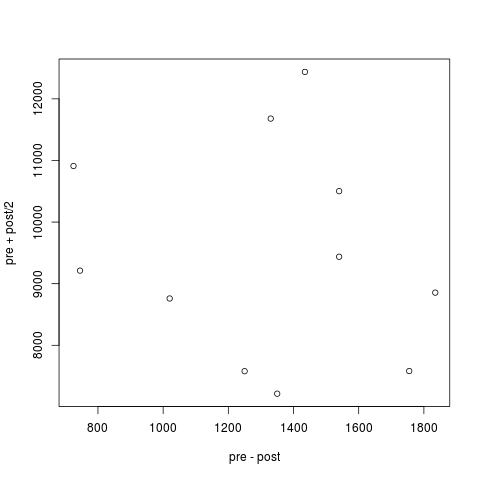
\includegraphics[width=1\textwidth]{img/bland_altman}
\end{columns}
\end{frame}

\begin{frame}[fragile,singleframe]
  \frametitle{Paired Wilcoxon Test}
  \begin{itemize}
  \item The basic idea of the Paired Wilcoxon test is similar to the paired T-test;
  \item The ``rank of the differences'' is calculated; (so the size of the differences has a smaller effect)
  \end{itemize}
  \begin{block}{}
{\small
\begin{verbatim}
> wilcox.test(pre,post,paired=T)

        Wilcoxon signed rank test with continuity correction

data:  pre and post 
V = 66, p-value = 0.00384
alternative hypothesis: true location shift is 
                        not equal to 0 

Warning message:
In wilcox.test.default(pre, post, paired = T) :
  cannot compute exact p-value with ties
\end{verbatim}}
  \end{block}
\end{frame}

\begin{frame}
  \frametitle{Paired Testing: Examples}
  Can anyone give me examples from your research of paired testing?
\end{frame}

%%%%%%%%%%%%%%%%%%%%%%%%%%%%%%%%%%%%%%%%%%%%%%%%%%%%%%%%%%%%%%%%%%%%%%%%%%%%%%%%%%


\section{Analysis of Variance} %(Chapter 7)
\subsection{Introduction}

\begin{frame}
  \begin{center}
    Part II: Analysis of Variance (ANOVA)
  \end{center}
\end{frame}

\begin{frame}
  \frametitle{Analysis of Variance}
  \begin{block}{Introduction}
    The Analysis of Variance (ANOVA) is a statistical method for
    testing many samples at the same time.
  \end{block}
  \begin{itemize}
  \item We want to find the best values for 4 parameters in our
    method. Each parameter can be valued between 0.0 and 1.0;
  \item Can we experiment the parameter values two at a time? Why? Why
    not?
  \end{itemize}
\end{frame}

\begin{frame}
  \frametitle{Analysis of Variance (Model)}
  \begin{block}{}
    Let each observation $x_{ij}$ be the $j$-th observation in group
    $i$. We decompose this observation as:
  \end{block}
  \begin{equation*}
    x_{ij} = \bar{x} + (\bar{x_i} - \bar{x}) + (x_{ij} - \bar{x_i})
  \end{equation*}
  \begin{block}{}
    In other words, eath observation is composed by the grand average
    of all samples, plus the deviation of the group, plus the
    (independent) error of the sample.
  \end{block}
\end{frame}

\begin{frame}
  \frametitle{Analysis of Variance (Model)}
  \begin{itemize} 
  \item The Analysis of Variance starts from the assumption that
    the variance of all groups is the same;
  \item If this assumption holds, then we can compare the variance
    difference between groups to test the null hypothesis that
    ``All groups have the same mean'';
  \end{itemize}
  \begin{block}{}
    Although it is called Analysis of Variance, and the main
    calculations are based on the variance of the groups, the final
    goal is a hypothesis centered on the means of the groups.
  \end{block}
\end{frame}

\begin{frame}[fragile,singleframe]
  \frametitle{Analysis of Variance (Example -- 1)}
{\small
  \begin{block}{}
\begin{verbatim}
> attach(red.cell.folate)
> summary(red.cell.folate)
folate          ventilation
Min.   :206.0   N2O+O2,24h:8   
1st Qu.:249.5   N2O+O2,op :9   
Median :274.0   O2,24h    :5   
Mean   :283.2                  
3rd Qu.:305.5                  
Max.   :392.0
\end{verbatim}
  \end{block}}

The red cell folate data set has three different categories: N20+02 24h, op, and O2 24h;

\end{frame}

\begin{frame}[fragile,singleframe]
  \frametitle{Analysis of Variance (Example -- 2)}

  \begin{block}{}
{\small
\begin{verbatim}
> anova(lm(folate~ventilation))
Analysis of Variance Table

Response: folate
            Df Sum Sq Mean Sq F value  Pr(>F)  
ventilation  2  15516  7757.9  3.7113 0.04359 *
Residuals   19  39716  2090.3                  
---
Signif. codes:  0 '***' 0.001 '**' 0.01 '*' 0.05 '.' 0.1 ' ' 1
\end{verbatim}}
  \end{block}
\begin{itemize}
  \item Sum Sq and Mean Sq show the variances calculated for the
    groups;
  \item The F statistic shows that the null hypothesis that all groups
    are the same;
\end{itemize}
\end{frame}

\begin{frame}[fragile,singleframe]
  \frametitle{Comparing multiple groups with ANOVA} 
{\smaller
  The F statistic in the Anova test tells us that not all groups are
  the same. How do we calculate the actuall differences betwee these
  groups?

  \begin{block}{}
\begin{verbatim}
> summary(lm(folate~ventilation))
Call:
lm(formula = folate ~ ventilation)

Residuals:
    Min      1Q  Median      3Q     Max 
-73.625 -35.361  -4.444  35.625  75.375 

Coefficients:
                     Estimate Std. Error t value Pr(>|t|)    
(Intercept)            316.62      16.16  19.588 4.65e-14 ***
ventilationN2O+O2,op   -60.18      22.22  -2.709   0.0139 *  
ventilationO2,24h      -38.62      26.06  -1.482   0.1548    
---
Signif. codes:  0 '***' 0.001 '**' 0.01 '*' 0.05 '.' 0.1 ' ' 1 

Residual standard error: 45.72 on 19 degrees of freedom
Multiple R-squared: 0.2809,     Adjusted R-squared: 0.2052 
F-statistic: 3.711 on 2 and 19 DF,  p-value: 0.04359
\end{verbatim}
  \end{block}}
\end{frame}

\begin{frame}[fragile,singleframe]
  \frametitle{Comparing multiple groups with ANOVA (2)}
  \begin{block}{}
{\small
\begin{verbatim}
    Coefficients:
                     Estimate Std. Error t value Pr(>|t|)    
(Intercept)            316.62      16.16  19.588 4.65e-14 ***
ventilationN2O+O2,op   -60.18      22.22  -2.709   0.0139 *  
ventilationO2,24h      -38.62      26.06  -1.482   0.1548    
---
Signif. codes:  0 '***' 0.001 '**' 0.01 '*' 0.05 '.' 0.1 ' ' 1
\end{verbatim}}
  \end{block}
  \begin{itemize}
  \item The Intercept is the \structure{mean of the first group} (N2O+02,24h);
  \item The Estimates are the \structure{differences} between the
    corresponding groups and the first;
  \item The \structure{Test Statistic} (last column), shows the
    p-value for the alternate hypothesis ``The mean of this group is
    different from the mean of the first group'';
  \item This version of the test compares only the first group (baseline) against all;
  \end{itemize}
\end{frame}

\begin{frame}[fragile,singleframe]
  \frametitle{Comparing multiple groups with ANOVA(3)}
  \begin{block}{Comparing All against All}
    As we increase the number of comparisons, we increase the chance
    of fininding a ``significant'' result. Therefore, our p-values
    must be adjusted to compensate for this.
  \end{block}
  \begin{block}{}
\begin{verbatim}
> pairwise.t.test(folate,ventilation)

    Pairwise comparisons using t tests with pooled SD 

data:  folate and ventilation 

      N2O+O2,24h N2O+O2,op
N2O+O2,op 0.042      -        
O2,24h    0.310      0.408    

P value adjustment method: holm
\end{verbatim}
  \end{block}
\end{frame}

\begin{frame}[fragile,singleframe]
  \frametitle{Non-parametric version}
  The Kruskal-Wallis test is the non-parametric counterpart of the one-way ANOVA:
  \begin{block}{}
{\small
\begin{verbatim}
> kruskal.test(folate~ventilation)

        Kruskal-Wallis rank sum test

data:  folate by ventilation 
Kruskal-Wallis chi-squared = 4.1852, df = 2, p-value = 0.1234
\end{verbatim}}
  \end{block}
\end{frame}

%%%%%%%%%%%%%%%%%%%%%%%%%%%%%%%%%%%%%%%%%%%%%%%%%%%%%%%%%%%%%%%%%%%%%%%%%%%%%%%%%%%%%%%%
% Former Class 8 - Selecting models

\section{Experimental Models}
\subsection{What are Experimental Models?}
\begin{frame}
  \frametitle{Experimental Models}
  When executing an experiment, we have to make many choices:
  \begin{itemize}
  \item What parameter values?
  \item How many repetitions?
  \item How many samples?
  \item Which data combinations?
  \end{itemize}
  The answers for these questions will be your \structure{Experimental Model}
\end{frame}

\begin{frame}
  \frametitle{First choice on Experimental Design}
  \begin{block}{}
    Before we can make any choices in the experimental design, you
    must decide: \structure{What is the goal of your experiment?}
  \end{block}
  \begin{itemize}
  \item Discover the influence of parameters (Sensibility Analysis);
  \item Find out best parameter values;
  \item Analyze one particular factor;
  \item Compare multiple methods;
  \item Test performance in data;
  \end{itemize}
\end{frame}

\subsection{Completely Randomized Design}
\begin{frame}
  \frametitle{The Completely Randomized Design (1)} 

  \begin{itemize}
  \item The most basic (and yet most important) experiment design pattern is
    the ``Completely Randomized Design'' (CRD).
  \item When we are not interested in any of the factors (Pilot Experiments)
  \item \alert{Attention: If we are not interested in the factors, we
        are not interested in the results for those factors!}
  \item We want to reduce the effects of factors in our results
  \end{itemize}
\end{frame}

\begin{frame}
  \frametitle{The Completely Randomized Design (2)}
  \begin{block}{Selecting Values}
    \begin{itemize}
    \item We distribute the repetitions (samples) randomly between all
      factors.
    \item \alert{However} a purely random distribution will tend to
      overrepresent some factor combinations over others;
    \item \structure{The Latin Hypercube} can be used to evenly
      distribute experiments among factors;
    \end{itemize}
  \end{block}
\end{frame}

\subsection{Latin Hypercube}

\begin{frame}
  \frametitle{Selecting Levels and Parameters}
  \begin{block}{The Latin HyperCube Sampling (LHS)}
    The LHS is a strategy for generating a random, robust parameter
    set from a large number of dimensions.
  \end{block}
  \begin{itemize}
  \item Define the desired number of experimental runs $k$, and the
    number of parameter (dimensions) $n$;
  \item For each parameter $x_i$, divide the range of that parameter
    into $k$ parts of equal size;
  \item The range of all $n$ parameters are arranged in a hypercube;
  \item Choose $k$ sets of parameters so that for each ``row'' and
    ``column'' in the hypercube there is only one sample;
  \end{itemize}
\end{frame}

\begin{frame}
  \frametitle{Selecting Levels and Parameters (2)}
  \begin{columns}[c]
    \column{0.6\textwidth}
    \begin{block}{When to use LHS}
      \begin{itemize}
      \item As a initial exploration of the parameter space;
      \item You are interested in seeing if there is a change in
        performance, but you don't know where to look;
      \item You want to show that your model/method is resistant to
        change in parameters;
      \item You want to concentrate on one parameter (not included in
        LHS), but don't care about the others;
      \end{itemize}
    \end{block}
    \begin{block}{When NOT to use LHS}
      \begin{itemize}
      \item You want to study the sensibility of one particular
        parameter;
      \end{itemize}
    \end{block}
    \column{0.3\textwidth}
    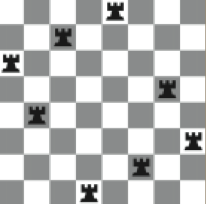
\includegraphics[width=1\textwidth]{img/lhs_chess}
  \end{columns}
\end{frame}

\subsection{Fixed Effect Model}

\begin{frame}
  \frametitle{Fixed Effect Model} 
  Based on \structure{domain knowledge}, we may decide to fix the
  values for some factors we know to be of interest.

  \begin{itemize}
  \item \structure{Fixed Effects:} Parameter values fixed by domain
    knowledge -- not relevant, or a single relevant level.
  \item \structure{Random Effects:} Parameter values which we don't
    want to interfere in the result;
  \item \structure{Observed Effects:} Calculated changes in levels to
    observe desired results;
  \end{itemize}

  Analysis of Variance (ANOVA) can be used on the observed levels to
  find significant trends in the results;
\end{frame}


%%%%%%%%%%%%%%%%%%%%%%%%%%%%%%%%%%%%%%%%
\subsection{Blocking Model}
\begin{frame}
  \frametitle{Randomized Complete Block Design (RCBD)} 

  In the analysis of Completely Random Design (CRD), observations are
  assigned to different \structure{Experimental Units}

  \begin{block}{Experimental Unit}
    A set of parameter values for an experiment
  \end{block}

  Sometimes an effect is \structure{not relevant} -- so we want to
  remove its influence from the experiment. But its value influences
  the result, so we can't just randomize it away.
\end{frame}

\begin{frame}
  \frametitle{Blocking Model} 
  {\small
  When these factors are known and controllable, an elegant way to
  reduce their effect in the experiment is by \structure{blocking}.

  Blocking consists of separating the experiments into
  \structure{blocks}, according with the levels of the experimental
  factor that we want to isolate.

  }
\end{frame}

\begin{frame}
  \frametitle{Blocking Example (1)}
  \begin{block}{Optimization Problems}
    \begin{columns}[c]
      \column{0.8\textwidth}
      A researcher develops a new algorithm for the optimization of
      time-series prediction models. He wants to test the performance of
      his model against recent algorithms in a variety of problems:
      Weather data, Financial data, Sun Radiation data, etc.
      \column{0.2\textwidth}
      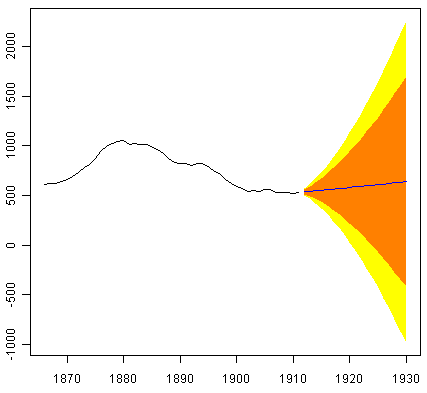
\includegraphics[width=1\textwidth]{img/timeseries}
    \end{columns}
  \end{block}
  \begin{itemize}
  \item The performance on each problem is not of interest (as opposed
    to the comparison with the other method);
  \item On the other hand, the performance is influenced by the
    problem type;
  \item We \structure{block} the problem type, by separating the
    experiment into subgroups based on the data set, and analyzing the
    results as paired samples;
  \end{itemize}
\end{frame}

\begin{frame}
  \frametitle{Blocking Example (2)}
  \begin{block}{Optimization Problems}
    \begin{columns}[c]
      \column{0.8\textwidth}
      A researcher develops a new algorithm for the optimization of
      time-series prediction models. He wants to test the performance of
      his model against recent algorithms in a variety of problems:
      Weather data, Financial data, Sun Radiation data, etc.
      \column{0.2\textwidth}
      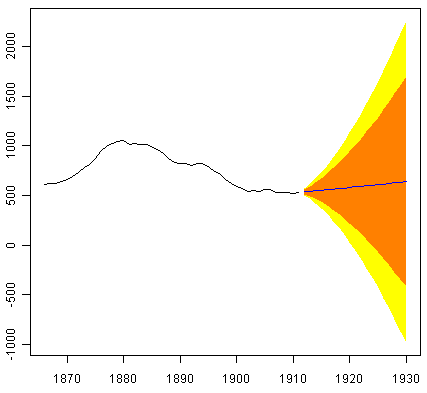
\includegraphics[width=1\textwidth]{img/timeseries}
    \end{columns}
  \end{block}
  \begin{itemize}
  \item Remember that $\mu_{\text{global}} = \mu_{0} + \mu_{\text{factor}}$
  \item If we employ \structure{Complete Randomization (CRD)} in this
    problem, the experimental error will also contain the variability
    from the different data sets;
  \item Since we can control the allocation of the data sets, we can
    group the experiments according to the problem in a sistematic
    way, to isolate the error due to the different data sets;
  \end{itemize}
\end{frame}

\begin{frame}
  \frametitle{Blocking x Randomization} 

  When we randomize the run order of our observations, we are guarding
  against unknown factors that may affect our results.

  Blocking comes into play whenever we know, from the beginning, that
  certain factors can influence our response variable. And we know
  that we are not interested in this influence.

  Examples:
  \begin{itemize}
  \item The effects of different benchmark in algorithm related research;
  \item The effects of different batches of materials in the experiment;
  \end{itemize}

\end{frame}

\begin{frame}
  \frametitle{Blocking Analysis (1)}
  \begin{block}{}
    In the general case, we have $a$ levels of the experimental
    factor, and $b$ levels of the blocking variable.
  \end{block}
  Our statistical model would be:
  \begin{equation*}
    y_{ij} = \mu + \tau_i + \beta_j + \epsilon_{ij} (i = 1\ldots a, j = 1\ldots b)
  \end{equation*}

  As seen in the last class for ANOVA, $\tau$ and $\beta$ are the
  group errors for the factors, and $\epsilon$ are the individual Errors.
\end{frame}

\begin{frame}
  \frametitle{Blocking Analysis (2)}
  \begin{block}{Null Hypothesis}
    We are interested in the experimental variable, $a$. Therefore,
    our null hypothesis is that:
    \begin{equation*}
      H_0: \sum{\tau_i} = 0 (\text{for} i = 0\ldots a)
    \end{equation*}
  \end{block}
  \begin{block}{Statistical Relevance of Blocking}
    It might be interesting to also test the statistical significance
    of the difference between blocks. The null hypothesis would be:
    \begin{equation*}
      H_0^b: \sum{\beta_j} = 0
    \end{equation*}
    Even if we are not interested in the effects of blocking --
    testing for the significance of the difference tells us if
    blocking is necessary or not.
  \end{block}
\end{frame}

\begin{frame}
  \frametitle{Blocking Analysis (3)}
  \begin{block}{Merging Blocks}
    Suppose that there are more than one factor that we are
    interesting in blocking. As long as we are not interested in the
    blocked effects (if we were, we wouldn't be blocking), we can
    merge the multiple factors into a single block factor.
  \end{block}
  \begin{block}{Example}
    In the previous experiment, we want to block our algorithms by
    different \emph{problem types} and different \emph{Data Set
      Lengths}. Although these are different factors, we can block
    them together into mixed factors.
  \end{block}
\end{frame}

\begin{frame}
  \frametitle{Blocking Analysis (4)}
  \begin{block}{Blocking Efficiency}
    We can calculate the \structure{Blocking Efficiency}, which shows
    how much larger a Complete Random Design would have to be to reach
    the same power as a Random Complete Block Design.
  \end{block}
  \begin{equation*}
    E = \frac{(b-1),MS_{blocks}+b(a-1)MS_E}{(ab-1)MS_E}
  \end{equation*}
  A value of 1.3, for example, would indicate that an CRD would need
  30\% more observations to achieve the same power.
\end{frame}

\begin{frame}[simpleframe,fragile]
  \frametitle{Blocking Example (1)}
  \begin{block}{}
    An student tries four different algorithms to the Capacitated
    Vehicle Routing Problem (CVRP1). These algorithms are compared by
    their application to 26 different benchmark problem instances. We
    want to compare their performances while blocking the effect of
    the problem instances.
  \end{block}

  \begin{columns}[c]
    \column{0.7\textwidth}
{\smaller
\begin{verbatim}
> data = read.table("cvrp.txt", header=T)
> data$Instance <- as.factor(data$Instance)
> with(data,boxplot(Result~Algorithm,
       xlab="Algorithm",ylab="Result",cex.lab=1.8))
\end{verbatim}}
    \column{0.3\textwidth}
    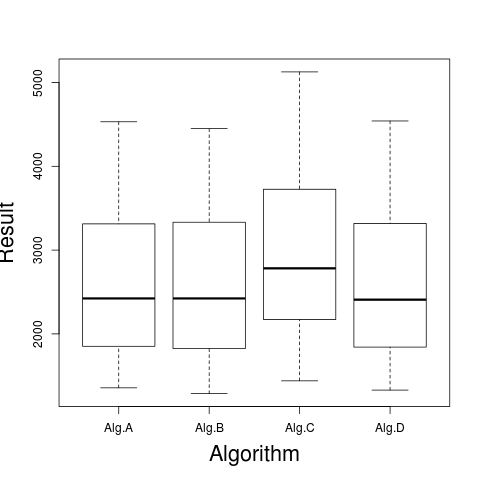
\includegraphics[width=1\textwidth]{img/cvrp1}
  \end{columns}
\end{frame}

\begin{frame}[simpleframe,fragile]
  \frametitle{Blocking Example (2)}
  \begin{center}
    Graphical Analysis of the Data\\
    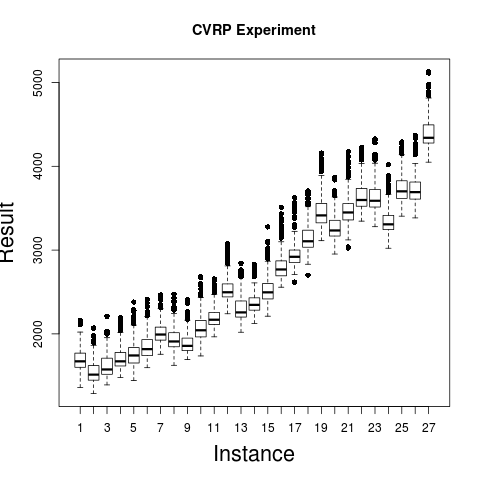
\includegraphics[width=0.4\textwidth]{img/cvrp2}
  \end{center}
{\small
\begin{verbatim}
with(data,boxplot(Result~Instance, xlab="Instance", ylab="Result", 
     main="CVRP Experiment", cex.lab=1.8,pch=16))
\end{verbatim}}
\begin{block}{}
  We can see clearly the influence of the different instances
\end{block}
\end{frame}

\begin{frame}[simpleframe,fragile]
  \frametitle{Blocking Example (2)}
  \begin{center}
    Graphical Analysis of the Data\\
    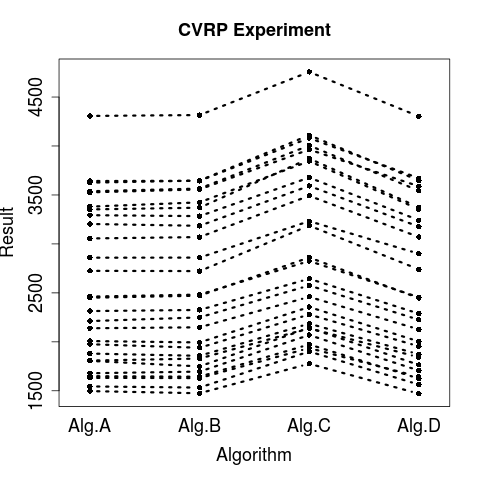
\includegraphics[width=0.3\textwidth]{img/cvrp3}
  \end{center}
{\small
\begin{verbatim}
> with(data,interaction.plot(Algorithm,Instance,Result,
  xlab="Algorithm",ylab="Result", main="CVRP Experiment",
  lwd=3,cex.lab=1.5,cex.axis=1.5,cex.main=1.5,legend=F,
  type="b",pch=16,lty=3))
\end{verbatim}}
\begin{block}{}
  The influence of the instances seems consistent with the Algorithm Factor
\end{block}
\end{frame}

\begin{frame}[simpleframe,fragile]
  \frametitle{Blocking Example (3)}
{\small
  \begin{block}{}
    Statistical model fit:
  \end{block}
\begin{verbatim}
> model.blocks<-aov(Result~Algorithm+Instance,data=data)
> summary(model.blocks)
Df Sum Sq Mean Sq F value Pr(>F)
Algorithm 3 2967410 989137 916.5 <2e-16 ***
Instance 26 71386444 2745632 2543.9 <2e-16 ***
Residuals 78 84186 1079 
---
\end{verbatim}
Significant effects for both the experimental and blocking factors. The
blocking efficiency is given by:
\begin{verbatim}
> b<-27; a<-4; MSb<-2745632; MSe<-1079
> ((b-1)*MSb + b*(a-1)*MSe)/((a*b-1)*MSe)
[1] 618.8988
\end{verbatim}
suggesting that it was a very good decision to include blocking in this
experimental design.}
\end{frame}

\begin{frame}
  \frametitle{Blocking Example (3)} 

  Now that we have our data of interest, we can apply sequential
  t.tests(ANOVA), to understand the relationship between the attibutes
  of interest.
\end{frame}

%%%%%%%%%%%%%%%%%%%%%%%%%%%%%%%%%%%%%%%%%%
\subsection{Factorial Model}
\begin{frame}
  \frametitle{Factorial Designs}
  \begin{block}{}
    In many experiments, we are interested in multiple factors:
    \begin{itemize}
    \item Multiple Parameters;
    \item Multiple Algorithms;
    \item Multiple Data Sets;
    \end{itemize}
    Using a \structure{Factorial Design} we can try to measure all
    effect combinations.
  \end{block}
  \begin{block}{Important Concepts}
    \begin{itemize}
    \item \structure{Main Effect}: Change of the response variable
      based on changes in one factor;
    \item \structure{Interaction Effect}: Change of the response
      variable based on simultaneous changes of two or more factors;
    \end{itemize}
  \end{block}
\end{frame}

\begin{frame}
  \frametitle{Factorial Design Example (1)} 
  \begin{block}{Experiment Outline}
    Two students wish to investigate factors that affect the
    electricity demand of an industrial fan.
  \end{block}
  \begin{block}{}
    From previous experiments, they determined that there are two
    factors which are likely candidates to explain the variability:
    \structure{Manufacturer} (A or B), and \structure{State} (normal
    or rewinded) of the motor.
  \end{block}
\end{frame}

\begin{frame}[simpleframe,fragile]
  \frametitle{Factorial Design Example (2)}
  \begin{center}
    Initial Data Visualization
  \end{center}
{\small
\begin{verbatim}
> with(data,boxplot(Current~State*Manufacturer, xlab="Group", 
       ylab="Current (A)", main="Motors Experiment", 
       cex.lab=1.8,pch=16))
\end{verbatim}
}

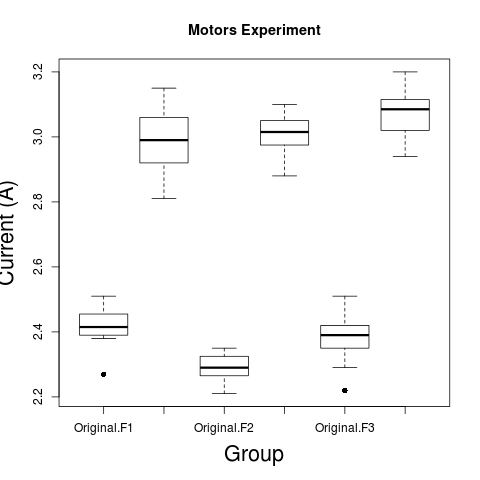
\includegraphics[width=0.5\textwidth]{img/fatorial1}

\end{frame}

\begin{frame}[simpleframe,fragile]
  \frametitle{Factorial Design Example (3)}
  \begin{center}
    Initial Data Visualization
  \end{center}
{\small
\begin{verbatim}
> with(data,interaction.plot(Manufacturer,State,Current, 
       xlab="Manufacturer", ylab="Current (A)", 
       main="Motors Experiment", cex.lab=1.8,lwd=3,
       type="b",pch=c(15,16),cex=2))
\end{verbatim}
}
\begin{columns}[c]
  \column{0.5\textwidth}
  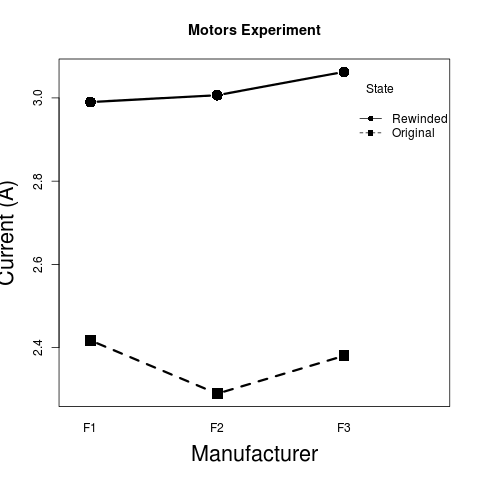
\includegraphics[width=1\textwidth]{img/fatorial2}
  \column{0.5\textwidth}
  \begin{itemize}
  \item Can we see any sort of iteraction or influence between the factors?
  \item We don't know! Need to investigate via experiment.
  \end{itemize}
\end{columns}
\end{frame}

\begin{frame}
  \frametitle{General Test Statistic for Factorial Design}
  \begin{itemize}
    \item $a$ levels for factor A;
    \item $b$ levels for factor B;
    \item $n$ samples for each combination of levels;
    \item Completely randomized combination of other factors;
  \end{itemize}
  \begin{equation*}
    y_{ijk} = \mu + \tau_i + \beta_j + (\tau\beta)_{ij} + \epsilon_{ijk}
  \end{equation*}
  Where $i = 1\dots a$, $j = 1\dots b$, $k = 1\dots n$. As usual, Null
  hypothesis is that the group errors are equal to 0.
\end{frame}

\begin{frame}[simpleframe,fragile]
  \frametitle{General Test Statistic for Factorial Design}
  {\small
    \begin{block}{}
      If the usual assumptions are met, $MS_A/MS_E$ , $MS_B/MS_E$ ,
      and $MS_{AB}/MS_E$ are distributed under their null hypotheses as
      an F variable with their respective degrees of freedom, and the
      hypotheses can be tested in the usual manner (i.e., comparing
      the obtained value of $F_0$ against the critical value of $F_{0;df_1;df_2}$).
    \end{block}
\begin{verbatim}
> model<-aov(Current~State*Manufacturer,data=data)
> summary(model)
                    Df Sum Sq Mean Sq F value   Pr(>F)    
State                1 12.956  12.956 2798.41  < 2e-16 ***
Manufacturer         2  0.118   0.059   12.71 1.04e-05 ***
State:Manufacturer   2  0.114   0.057   12.27 1.49e-05 ***
Residuals          114  0.528   0.005
\end{verbatim}
  } 

If ANOVA indicates the existence of significant effects, these effects
must be investigated by further statistical testing. The standard R
functions discussed in last class can be used (one against all, all
agains all, etc).

\end{frame} 

% Anova adding the Interaction as a factor
% > model<-aov(Current~State*Manufacturer,data=data)
% > summary(model)

%%%%%%%
\section{Another Example}
\subsection{Another Example}
\begin{frame}
  \frametitle{Paper: Ant Colony Optimization with Immigrant Schemes for the DTSP}
  \begin{block}{Summary}
    Modifications to an ACO algorithm applied to a Dynamic Optimization Problem.
  \end{block}
  \begin{itemize}
  \item \structure{Section 2--6}: Introductions to the algorithms;
  \item \structure{Section 7.1}: Experimental Setup;
  \item \structure{Section 7.2}: Parameter Settings;
  \item \structure{Section 7.3}: Variation on the Data Sets;
  \item \structure{Section 7.4}: Variation on the Data Set Parameters;
  \item \structure{Section 7.5}: Analysis on solution diversity;
  \item \structure{Section 7.6}: Analysis of the ``traffic factor'' parameter;
  \item \structure{Section 7.7}: Comparison with other algorithms;
  \end{itemize}
\end{frame}

\begin{frame}
  \frametitle{Paper: Ant Colony Optimization with Immigrante Schemes for the DTSP}

  \begin{block}{}
    \emph{Ant Colony Optimization With Immigrants Schemes For The
      Dynamic Travelling Salesman Problem with Traffic Factors}\\
    Michalis MAvrovouniotis, Shengxiang Yang\\
    Applied Soft Computing 13(2013)4023--4037
  \end{block}
  
  \vfill

  Take a read at section 7 of this paper -- it is very instructive of
  Experimental design. \structure{It is not perfect!} Note the
  positive and the negative points of the experiment Design in this
  paper.
\end{frame}


\end{document}
